\documentclass[11pt,a4paper]{article}
\usepackage[margin=1in]{geometry}
\usepackage[T1]{fontenc}
\usepackage[utf8]{inputenc}
\usepackage{lmodern}
\usepackage{graphicx}
\usepackage{booktabs}
\usepackage{float}
\usepackage{hyperref}
\graphicspath{{figures/}{../figures/}}
\hypersetup{colorlinks=true,linkcolor=blue,urlcolor=blue}
\title{Four Questions from India's NFHS-6 Fact Sheets}
\author{Nakshatra Ghosh}
\date{30 September 2026}

\begin{document}
\maketitle

\begin{abstract}
This portfolio extracts 101 indicators for India and 35 States/Union
Territories from the 2023--24 National Family Health Survey (NFHS-6)
fact-sheet compendium. It investigates four area-level questions among the
27 states and adds a descriptive multivariate profile analysis. Larger
schooling and stunting gaps coexist, as do child-marriage and teenage-
motherhood gaps. Schooling and internet gender gaps are related less
strongly. Every state has both lower child stunting and higher women's
overweight than in NFHS-5, but the magnitudes of those two changes are not
related. Model comparisons use leave-one-state-out prediction errors.
No association is interpreted causally.
\end{abstract}

\section{Why these questions matter now}

The NFHS-6 India/State compendium was released in 2026 and gives the
latest published fact-sheet comparison with NFHS-5 for these measures.
At the India level, under-five stunting was still 29.3\% in NFHS-6,
despite a 6.2-percentage-point decline from NFHS-5. Women's overweight
or obesity rose from 24.0\% to 30.7\%. This motivates Q1 and Q4:
child undernutrition and adult excess weight can be present at the same
time, so focusing on only one outcome misses the breadth of nutrition
policy needs.

Child marriage among women aged 20--24 was 20.1\% in NFHS-6. The
teenage-motherhood-or-pregnancy indicator was 6.7\%. Their different
age cohorts rule out a direct individual-level transition analysis in
these tables, but Q2 can reveal whether the two geographic gaps appear
together. For Q3, 64.3\% of women and 80.5\% of men aged 15--49 had
ever used the internet. The 16.2-point national gender gap makes digital
access a current issue even as internet use rose markedly in both groups.
The project asks whether a schooling gap explains part of its geographic
variation rather than assuming that education is the only barrier.

\section{Data and design}

The source is the International Institute for Population Sciences (IIPS)
\emph{NFHS-6, 2023--24: India and State/UT Fact Sheets}.\footnote{\href{https://www.nfhsiips.in/nfhsuser/assets/National\%20Family\%20Health\%20Survey\%20\%28NFHS-6\%29\%202023-2024\%20Fact\%20Sheets.pdf}{IIPS NFHS-6 India/State fact-sheet PDF.}}
The extracted CSV has 3,636 area--indicator rows: 101 indicators for India
and 35 States/UTs. Manipur is absent. Each row contains NFHS-6 urban,
rural and total estimates, an NFHS-5 total, and its physical PDF page.
An asterisk suppresses an estimate based on fewer than 25 unweighted
cases; parentheses mark 25--49 cases. The extraction retains both marks.
These are published area averages, not individual-level microdata.

The regression sample is the 27 states. India is not an independent state
observation. Eight UTs are excluded because some have small or suppressed
rural cells. Every state receives equal weight. Household interview counts
would be invalid precision weights for outcomes based on narrower groups
such as children under five. The fact sheets lack the indicator-specific
sampling variances needed to carry NFHS sampling error into these models.
NFHS-6 fact-sheet estimates are described by IIPS as provisional.

For question $q$, let $x_s$ be the predictor and $y_s$ the outcome, both
in percentage points for state $s$. The explanatory summary is
\begin{equation}
y_s=\alpha+\beta x_s+\varepsilon_s.
\end{equation}
Ordinary least squares (OLS) gives an interpretable slope. HC3 robust
standard errors reduce dependence on constant residual variance in a
small cross-section. The reported 95\% intervals use the residual
degrees of freedom, but condition on published estimates as observed;
they are not full NFHS survey confidence intervals. Four questions were
examined, so their tests are exploratory rather than confirmatory.

\section{Model comparison and selection}

Each question uses four models: a mean-only benchmark, linear OLS,
quadratic OLS with one added curvature term, and Huber robust linear
regression. The quadratic checks curvature but
can overfit 27 observations. Huber checks whether large residuals drive
the slope. For each state in turn, we fit the model on the other 26 and
predict the held-out state. We compare root mean squared prediction
error across the 27 held-out predictions (LOO RMSE). BIC is saved for the
three OLS models; it is not compared to Huber's different loss.
LOO ranks prediction, not explanation or causality. A very small RMSE
advantage does not override the interpretability of a straight line.
Binomial logistic regression is not fitted because these published
percentages do not include the necessary individual counts and survey
weights.

\section{Four questions and answers}

\subsection{Q1: Schooling and child stunting gaps}
Indicator 12 is the percentage of women aged 15--49 with at least ten
years of schooling. Indicator 69 is under-five stunting: height-for-age
below two standard deviations on the WHO standard. The predictor is
urban minus rural schooling; the outcome is rural minus urban stunting.
Both are within-state gaps, reducing dependence on shared state levels
but leaving urban--rural confounding.

The mean state schooling gap is 19.16 points and the mean stunting gap
is 5.37 points. The OLS slope is 0.392 (95\% HC3 interval 0.170 to
0.614; $R^2=0.281$). A ten-point wider schooling gap is associated
with a 3.9-point wider stunting gap. Huber's slope is 0.412. Its
LOO RMSE is 5.15 versus 5.19 for linear OLS, a negligible predictive
gain. The linear estimate remains the main explanatory summary.
The women counted in schooling are not necessarily mothers of the
children counted in stunting.

\subsection{Q2: Child marriage and teenage motherhood gaps}
Indicator 16 measures women aged 20--24 married before 18. Indicator
19 measures women aged 15--19 already mothers or pregnant at interview.
Both predictor and outcome are rural minus urban gaps. The mean gaps
are 8.04 and 3.71 points, respectively. The OLS slope is 0.373
(95\% HC3 interval 0.181 to 0.566; $R^2=0.503$). Huber's slope
is 0.340 and its LOO RMSE is 2.82 versus 2.88 for linear OLS.
The quadratic predicts worse than either line. The indicators refer
to different cohorts, so this is geographic coexistence rather than
a causal marriage-to-pregnancy pathway.

\subsection{Q3: Schooling and internet-use gender gaps}
Indicators 12 and 13 measure women's and men's ten-year schooling
shares; indicators 14 and 15 measure whether they have ever used the
internet. Both gaps are men minus women, using NFHS-6 total estimates.
The mean state schooling gender gap is 5.74 points; the mean internet
gender gap is 13.83 points. The OLS slope is 0.653 (95\% HC3 interval
0.192 to 1.114; $R^2=0.232$). A quadratic has the smallest LOO RMSE,
6.57 versus 6.89 for linear OLS. Yet BIC is nearly tied: 187.04 for
linear and 187.09 for quadratic. There are few states at the largest
schooling gaps, so the apparent curvature is a lead to investigate,
not firm evidence of a nonlinear mechanism. The linear estimate remains
the main summary. Ever having used the internet does not measure
current access, frequency, skill or affordability.

\subsection{Q4: Declining stunting and rising overweight}
The predictor is the NFHS-5 minus NFHS-6 under-five stunting rate
(indicator 69); positive means a decline. The outcome is the NFHS-6
minus NFHS-5 overweight-or-obesity rate among women aged 15--49
(indicator 76); positive means an increase. Indicator 76 excludes
pregnant women and women with a birth in the preceding two months.
These measures refer to different populations.

All 27 states have positive values on both axes. The average stunting
decline is 5.88 points and the average overweight rise is 6.37 points.
The OLS slope is 0.105 (95\% HC3 interval -0.520 to 0.729;
$R^2=0.008$). The intercept-only benchmark has the smallest LOO
RMSE, 3.14 versus 3.33 for linear OLS. The finding is coexistence
of two trends, with no evidence here that faster improvement on one
predicts a faster rise in the other.

\begin{table}[H]
\centering
\caption{State-level linear OLS estimates; $n=27$ for each question}
\label{tab:estimates}
\begin{tabular}{lrrrr}
\toprule
Question & Slope & HC3 95\% interval & $R^2$ & Huber slope \\
\midrule
Q1 Schooling--stunting gaps & 0.392 & [0.170, 0.614] & 0.281 & 0.412 \\
Q2 Marriage--motherhood gaps & 0.373 & [0.181, 0.566] & 0.503 & 0.340 \\
Q3 Schooling--internet gender gaps & 0.653 & [0.192, 1.114] & 0.232 & 0.682 \\
Q4 Stunting decline--overweight rise & 0.105 & [-0.520, 0.729] & 0.008 & 0.113 \\
\bottomrule
\end{tabular}
\end{table}

\begin{table}[H]
\centering
\caption{LOO RMSE in percentage points; lower is better for prediction}
\label{tab:prediction}
\begin{tabular}{lrrrrl}
\toprule
Question & Mean only & Linear & Quadratic & Huber & Lowest RMSE \\
\midrule
Q1 & 5.96 & 5.19 & 5.23 & 5.15 & Huber \\
Q2 & 3.87 & 2.88 & 3.12 & 2.82 & Huber \\
Q3 & 7.62 & 6.89 & 6.57 & 6.95 & Quadratic \\
Q4 & 3.14 & 3.33 & 3.48 & 3.38 & Mean only \\
\bottomrule
\end{tabular}
\end{table}

\begin{figure}[H]
\centering
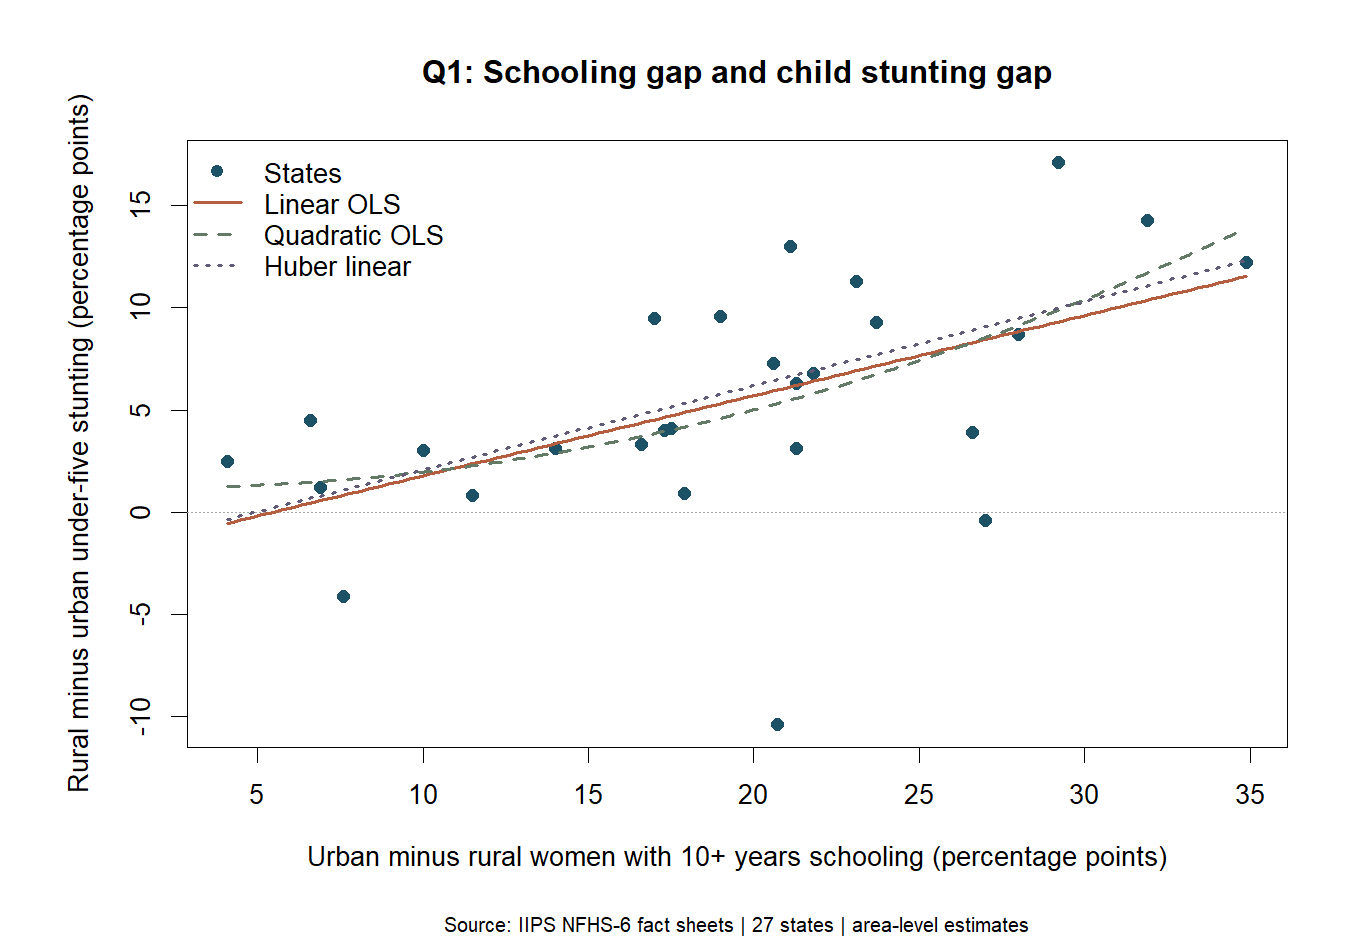
\includegraphics[width=.85\textwidth]{q1_schooling_stunting_scatter.png}
\caption{Rural--urban schooling and stunting gaps. Lines show linear,
quadratic and Huber fits; the source and units appear in the graph.}
\end{figure}

\begin{figure}[H]
\centering
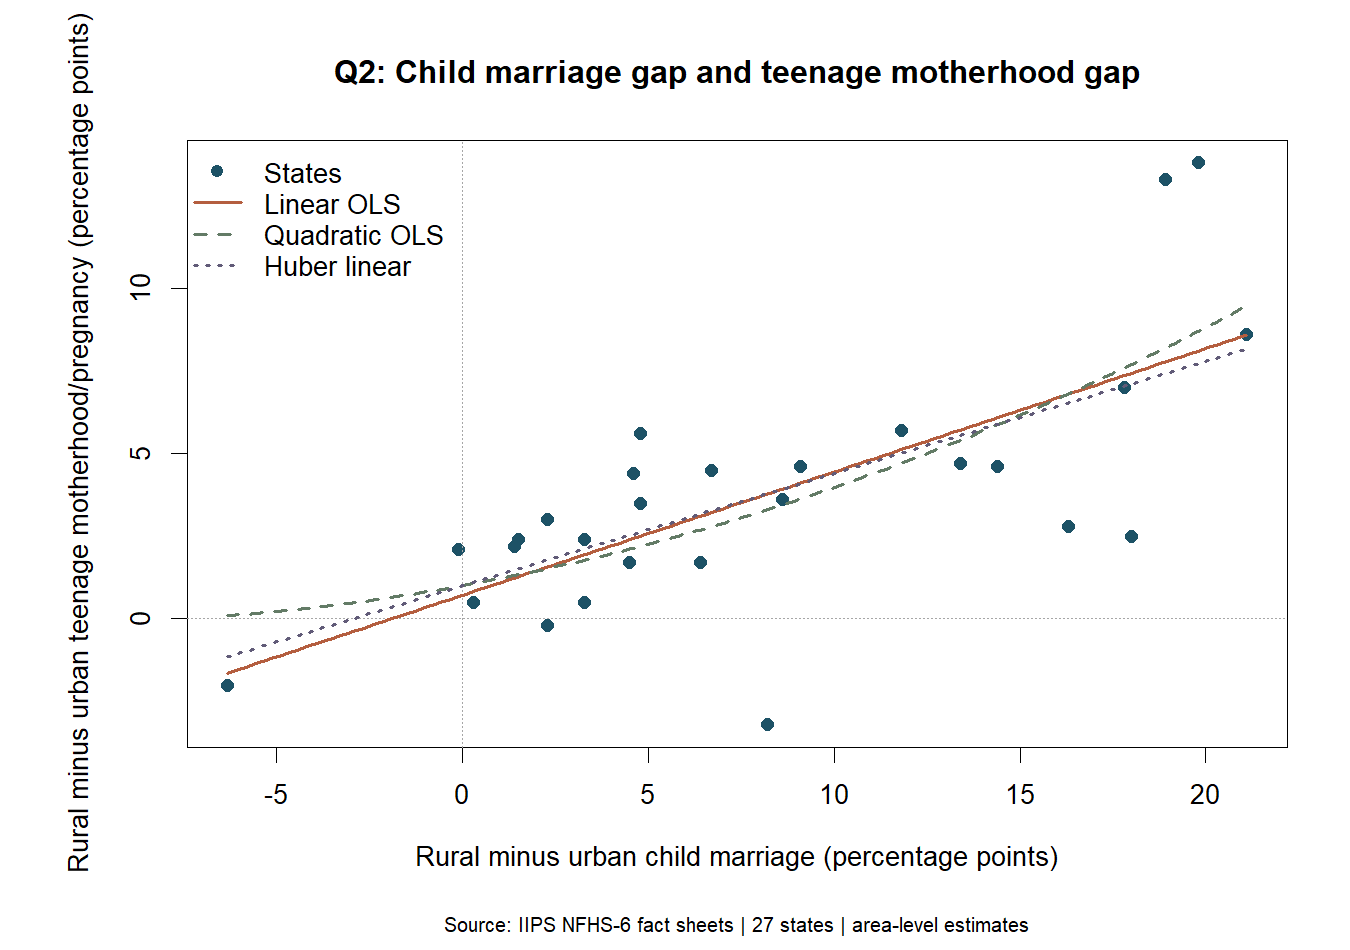
\includegraphics[width=.85\textwidth]{q2_marriage_motherhood_scatter.png}
\caption{Rural--urban gaps in child marriage and teenage motherhood or pregnancy.}
\end{figure}

\begin{figure}[H]
\centering
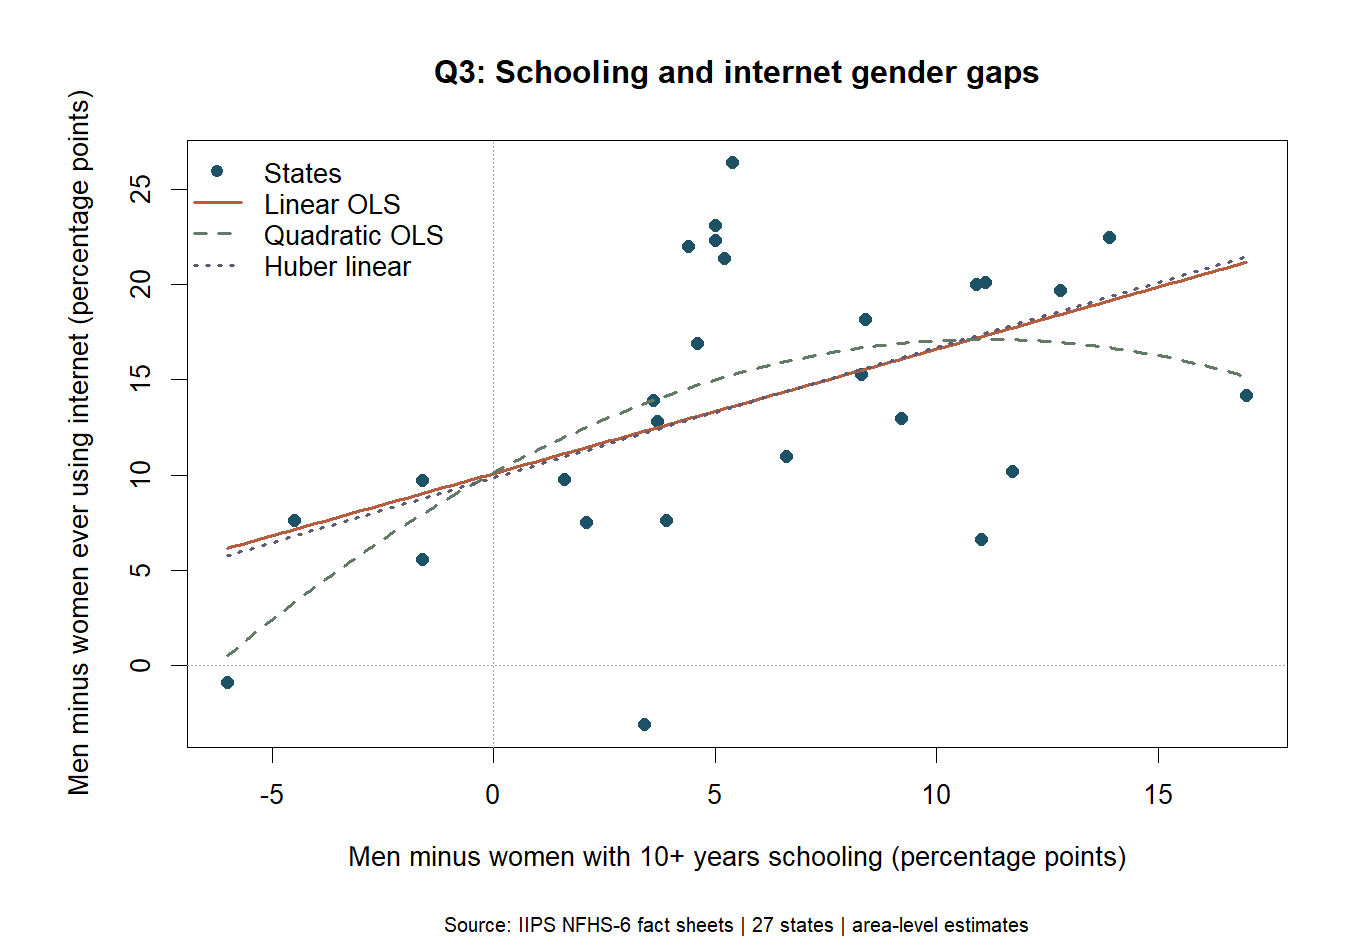
\includegraphics[width=.85\textwidth]{q3_digital_gender_scatter.png}
\caption{Gender gaps in schooling and internet ever-use.}
\end{figure}

\begin{figure}[H]
\centering
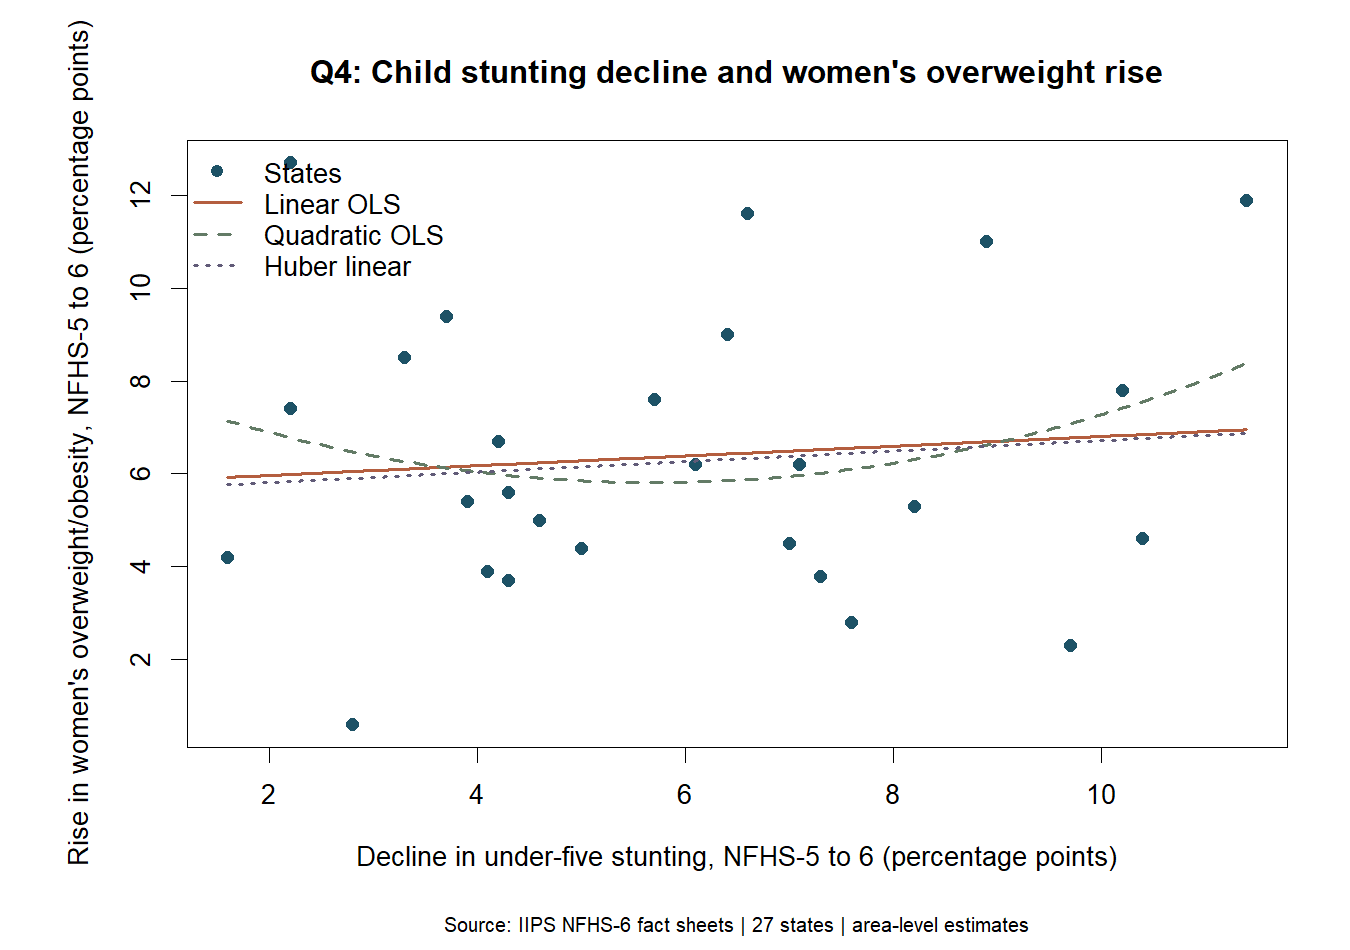
\includegraphics[width=.85\textwidth]{q4_nutrition_transition_scatter.png}
\caption{State changes in child stunting and women's overweight or obesity.
The association is near zero even though both changes occur in every state.}
\end{figure}

\clearpage
\subsection{Distributional and residual checks}

The predictor and outcome need not have matching marginal distributions.
Each is a different percentage-point quantity, and OLS describes the
mean outcome conditional on the predictor. Relevant diagnostics concern
the shape and spread of residuals, influential states and the stability
of the slope. The separate predictor and outcome histograms therefore
do not, by themselves, invalidate any regression.

The Q1 residuals have one unusual state: Sikkim's studentized residual
is -4.30, and a Shapiro--Wilk screening test gives $p=0.016$.
Leaving out any one state changes the Q1 linear slope only from 0.339
to 0.439, while Huber's slope is 0.412. For Q2, a one-predictor
Breusch--Pagan screening test suggests unequal residual spread
($p=0.028$). Its HC3 slope standard error is 0.094, compared with
0.074 under the constant-variance formula. The Q2 leave-one-state-out
slopes range from 0.316 to 0.414. These diagnostics support using HC3
and reporting Huber sensitivity, while keeping small-sample uncertainty
and the absence of survey sampling variances in view. The tests are
descriptive screens in only 27 states, not proof of model validity.

\begin{figure}[H]
\centering
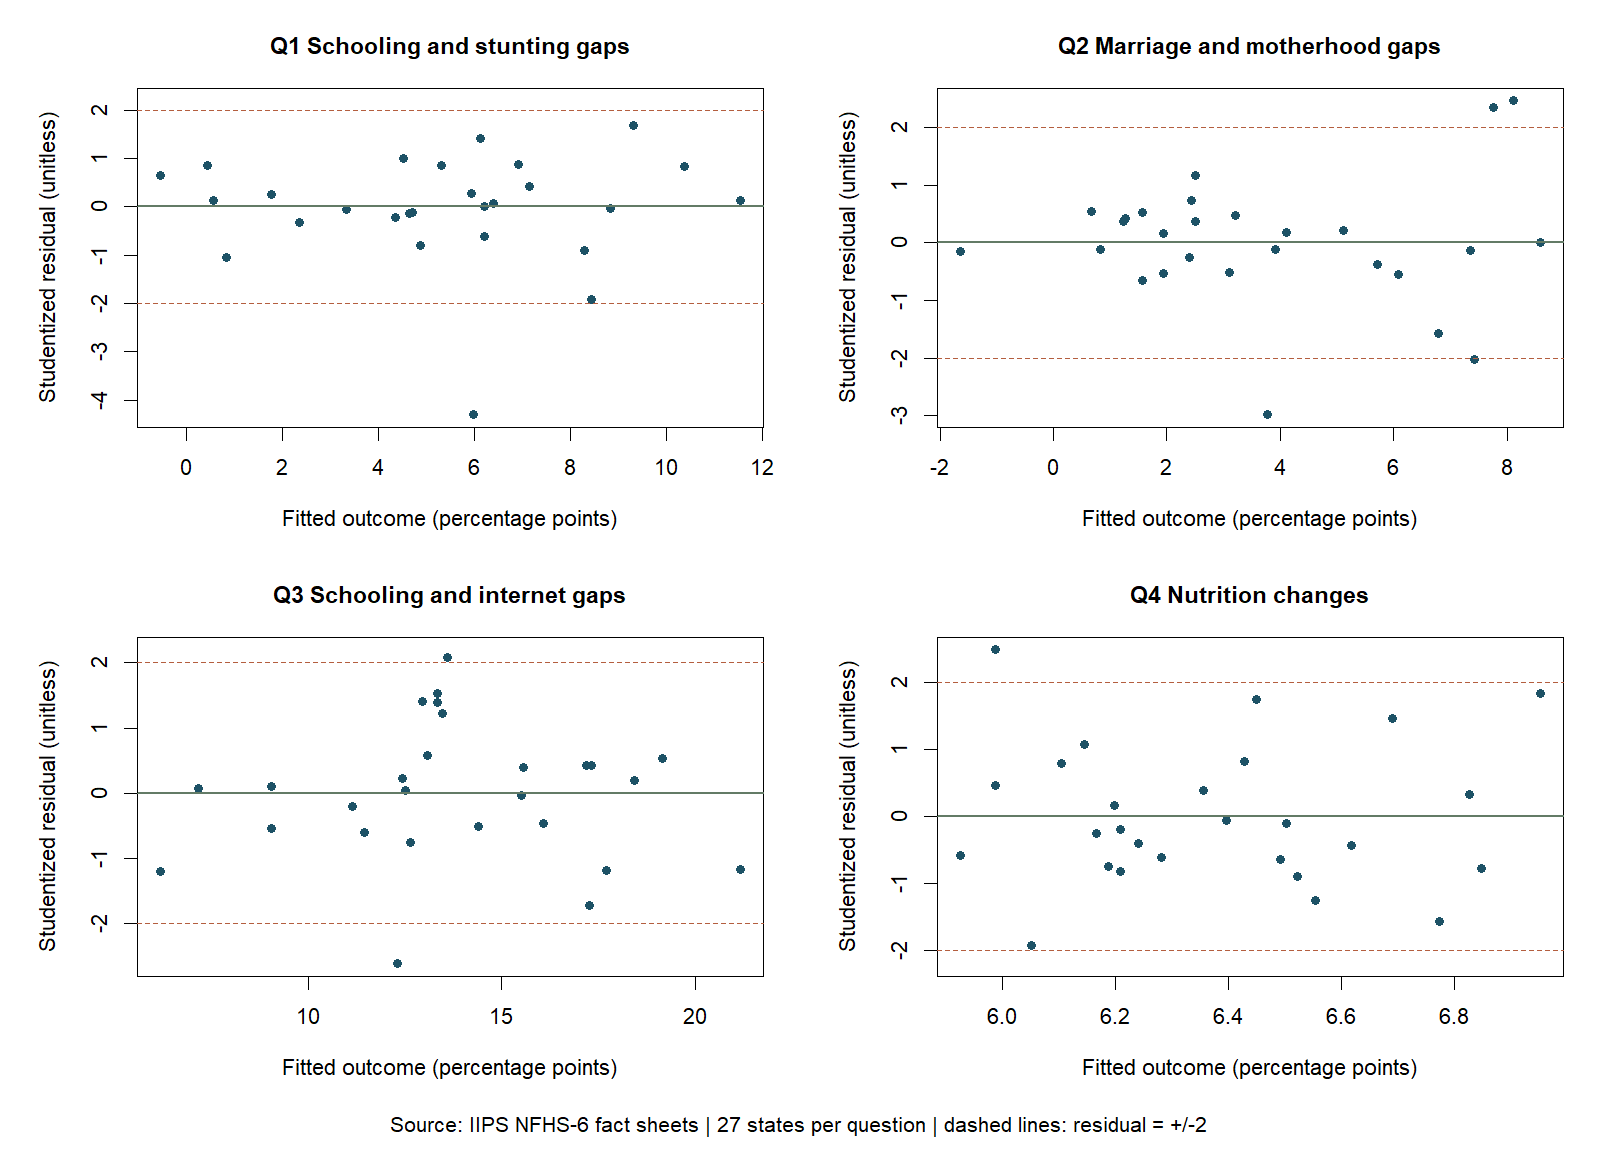
\includegraphics[width=.88\textwidth]{regression_residuals.png}
\caption{Studentized residuals against fitted values for the four linear
summaries. Dashed lines mark residuals of $\pm2$.}
\end{figure}

\begin{figure}[H]
\centering
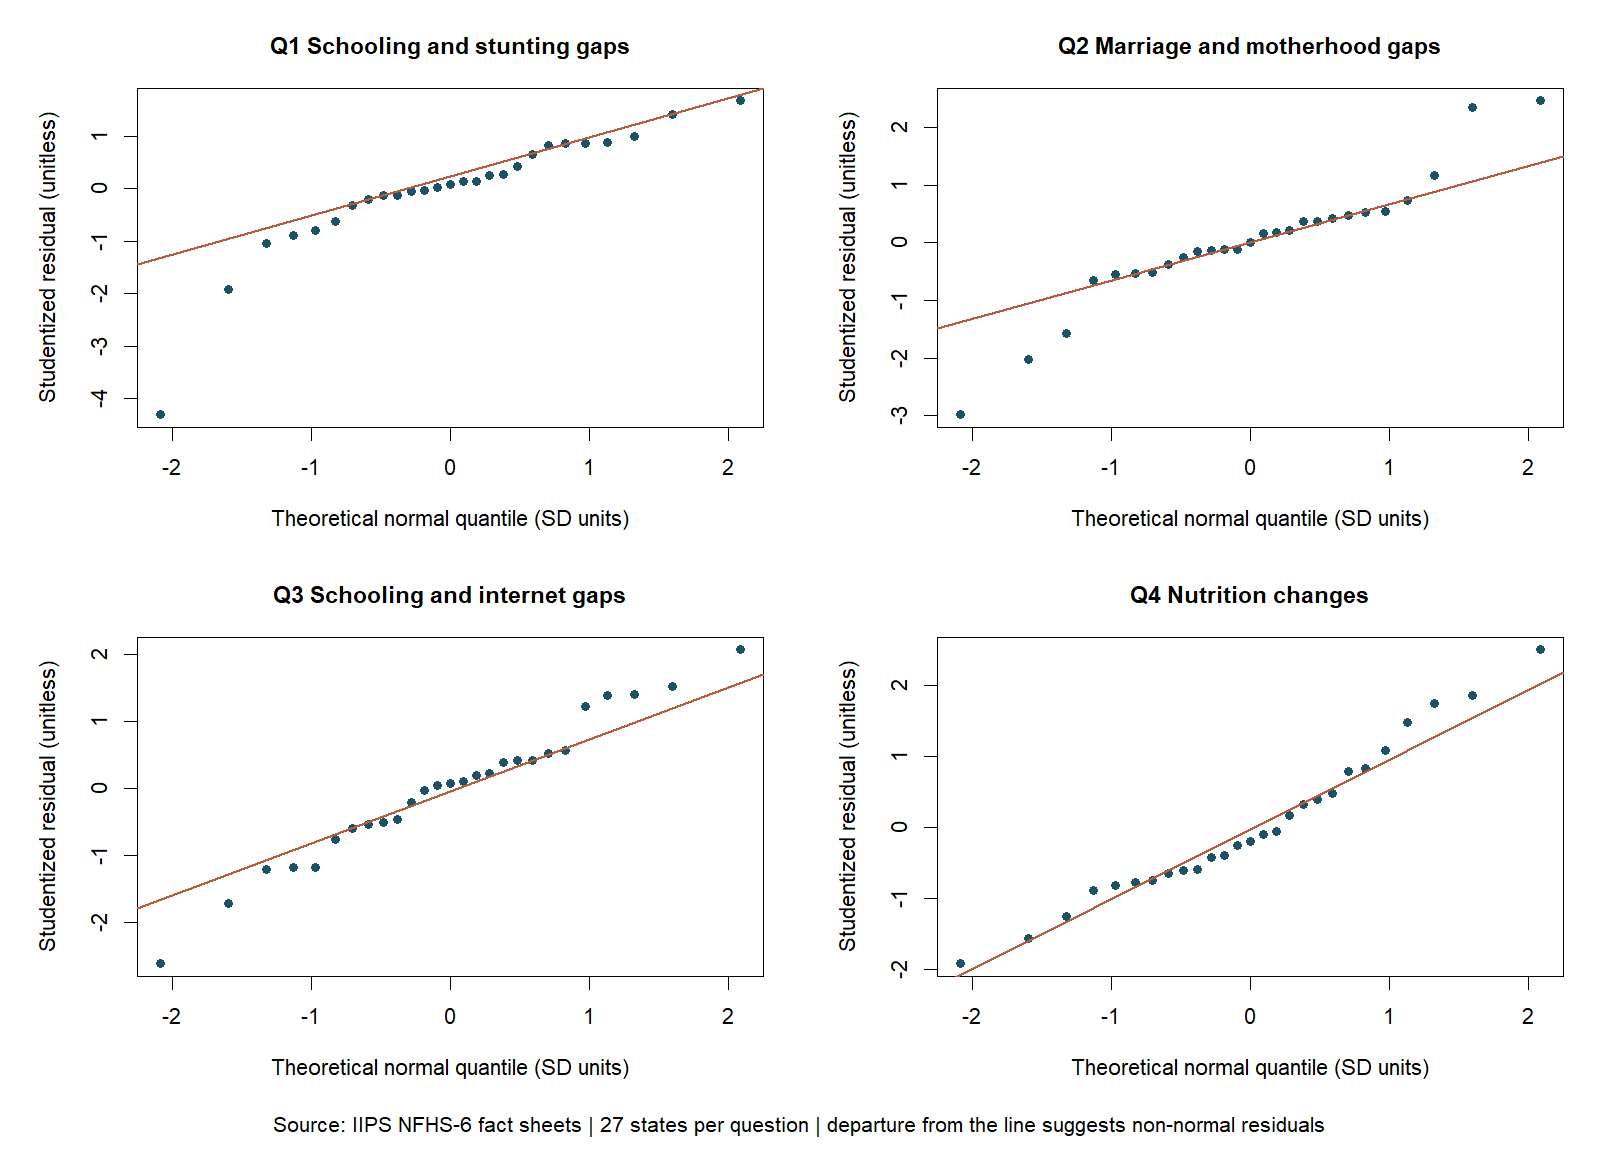
\includegraphics[width=.88\textwidth]{regression_residual_qq.png}
\caption{Normal quantile plots of studentized residuals. Q1's lower-tail
departure reflects the unusual Sikkim observation.}
\end{figure}

\section{Descriptive statistics}

Table~\ref{tab:description} describes the 27-state distributions
underlying each regression. The positive-count column shows whether
a gap or change is widespread rather than driven only by its mean.
The CSV also includes quartiles and each state's values.

\begin{table}[H]
\centering
\small
\caption{State descriptive statistics, in percentage points}
\label{tab:description}
\resizebox{\textwidth}{!}{%
\begin{tabular}{llrrrrrr}
\toprule
Question & Variable & Mean & Median & SD & Min & Max & Positive states \\
\midrule
Q1 & Schooling gap & 19.16 & 20.60 & 7.90 & 4.1 & 34.9 & 27 \\
Q1 & Stunting gap & 5.37 & 4.10 & 5.85 & -10.4 & 17.1 & 24 \\
Q2 & Child-marriage gap & 8.04 & 6.40 & 7.22 & -6.3 & 21.1 & 25 \\
Q2 & Teenage-motherhood gap & 3.71 & 3.00 & 3.80 & -3.2 & 13.8 & 24 \\
Q3 & Schooling gender gap & 5.74 & 5.00 & 5.52 & -6.0 & 17.0 & 23 \\
Q3 & Internet gender gap & 13.83 & 13.90 & 7.48 & -3.1 & 26.4 & 25 \\
Q4 & Stunting decline & 5.88 & 5.70 & 2.71 & 1.6 & 11.4 & 27 \\
Q4 & Women's overweight rise & 6.37 & 5.60 & 3.08 & 0.6 & 12.7 & 27 \\
\bottomrule
\end{tabular}
}
\end{table}

\begin{figure}[H]
\centering
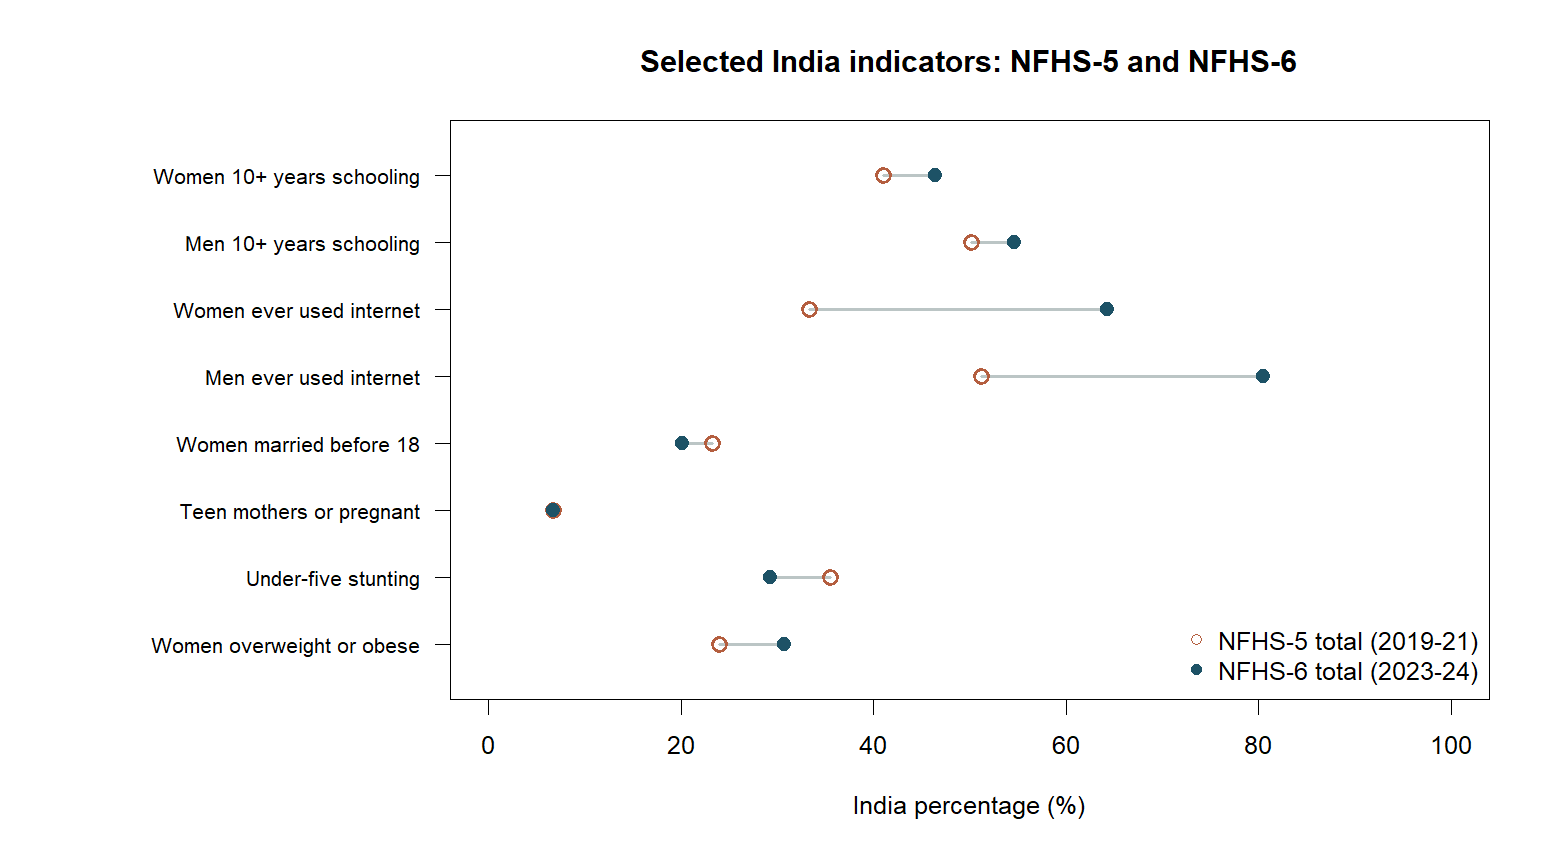
\includegraphics[width=.85\textwidth]{india_selected_changes.png}
\caption{Selected published India totals across NFHS-5 and NFHS-6.
Different rows have different eligible populations.}
\end{figure}

\begin{figure}[H]
\centering
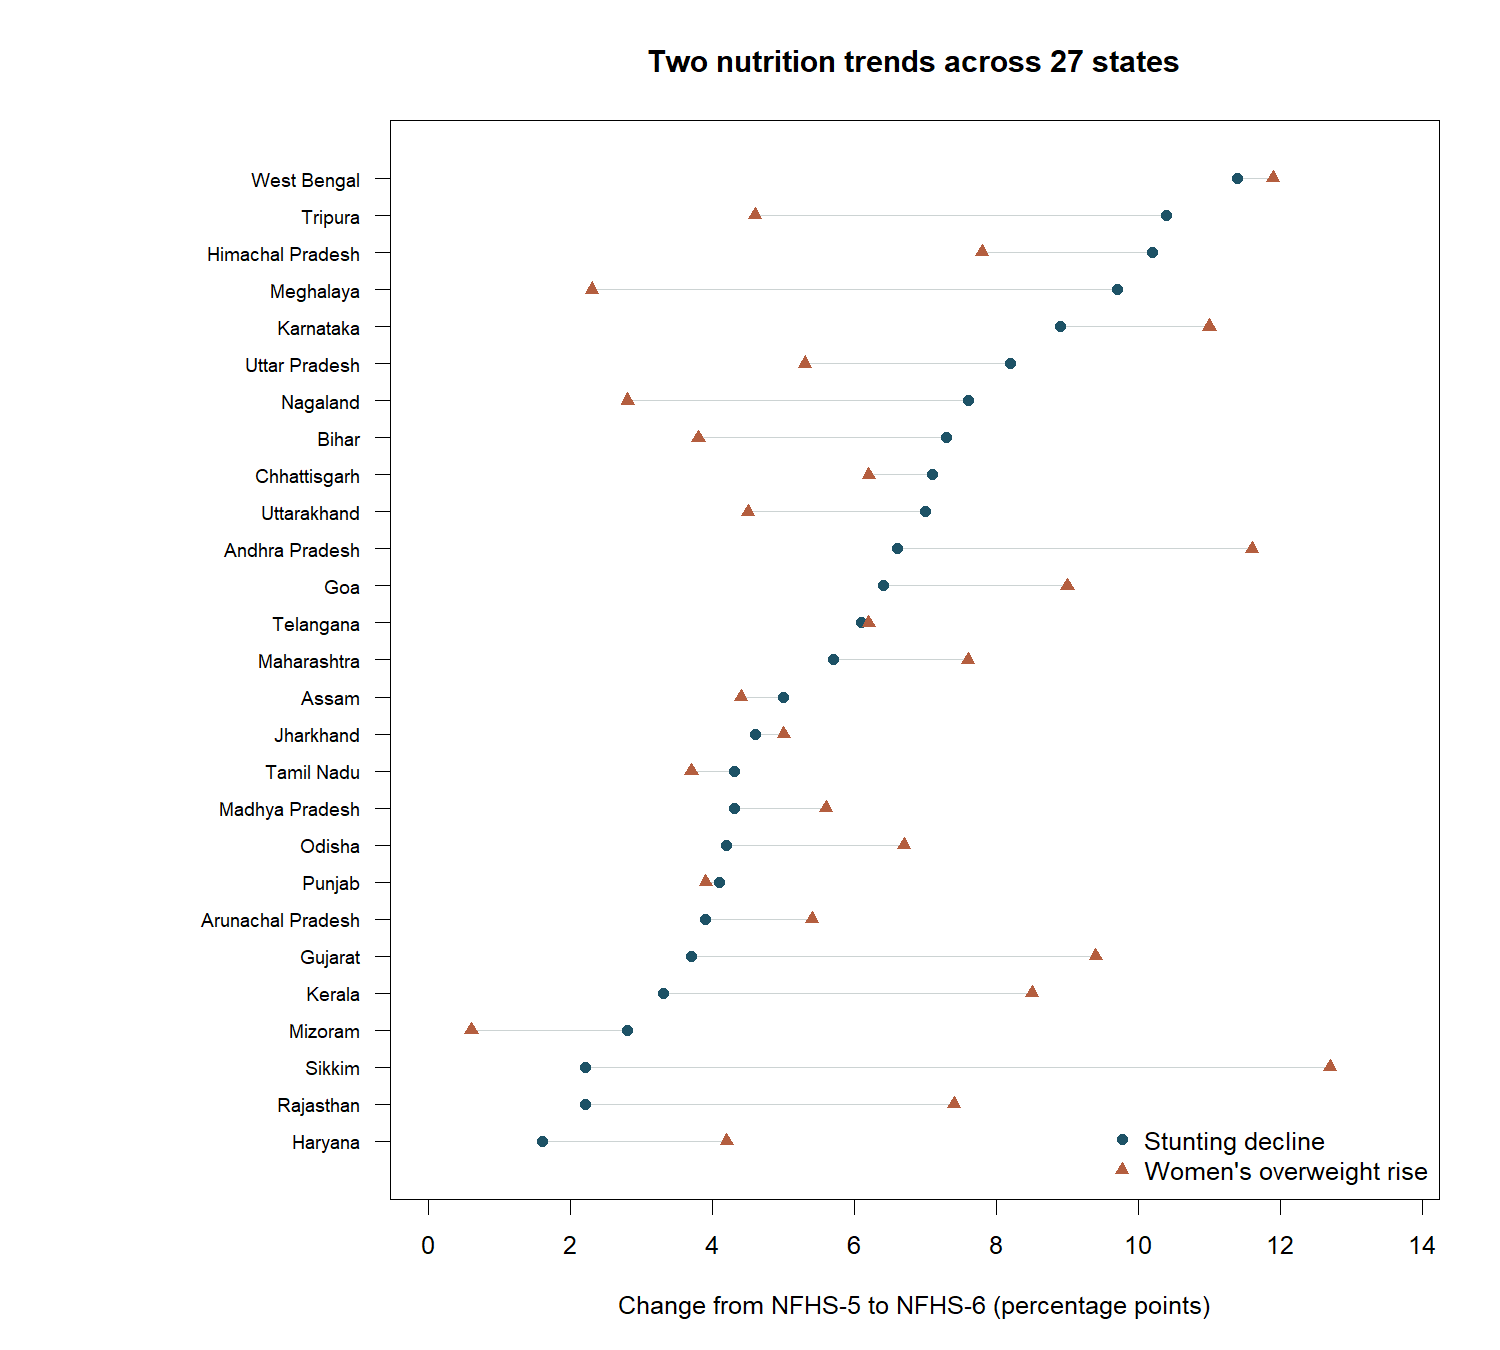
\includegraphics[width=.82\textwidth]{state_nutrition_changes.png}
\caption{Every state has a positive stunting decline and an increase in
women's overweight or obesity. Dot positions give percentage-point
changes; the outcomes use different populations.}
\end{figure}

\section{Exploratory multivariate state profiles}

The repository standardizes seven NFHS-6 state totals: women's
schooling, women's internet ever-use, child marriage, four or more
antenatal visits, adequate diet among children aged 6--23 months,
under-five stunting, and women's overweight or obesity. PCA describes
their correlation structure; k-means describes proximity among state
profiles. This is not a single development score and implies no
causal effect. Women's overweight is a health burden even though it
shares a positive first-component loading with schooling.

The Kaiser--Meyer--Olkin diagnostic is 0.740. The first two principal
components explain 59.2\% and 14.1\% of standardized variation.
A 500-repetition column-permutation benchmark places only the first
observed eigenvalue above its 95th-percentile null threshold. The
first component loads positively on women's schooling (0.460),
overweight (0.419), internet use (0.353), antenatal care (0.341)
and adequate child diet (0.306), and negatively on child stunting
(-0.396) and child marriage (-0.350). Its sign was oriented toward
schooling for readability. The minimum correlation of first-component
loadings after leaving out one state is 0.996.

K-means is fitted to all seven standardized variables, not to a
two-dimensional PCA display. Among $k=2,3,4$, the mean silhouette
is highest at $k=2$: 0.317 versus 0.249 and 0.247. The two groups
contain 12 and 15 states. Omitting one feature at a time and
reclustering yields a mean adjusted Rand index of 0.839; some
feature deletions change assignments. The silhouette indicates
moderate, not sharp, separation. Cluster labels are descriptive
and should not be treated as permanent rankings.

\begin{figure}[H]
\centering
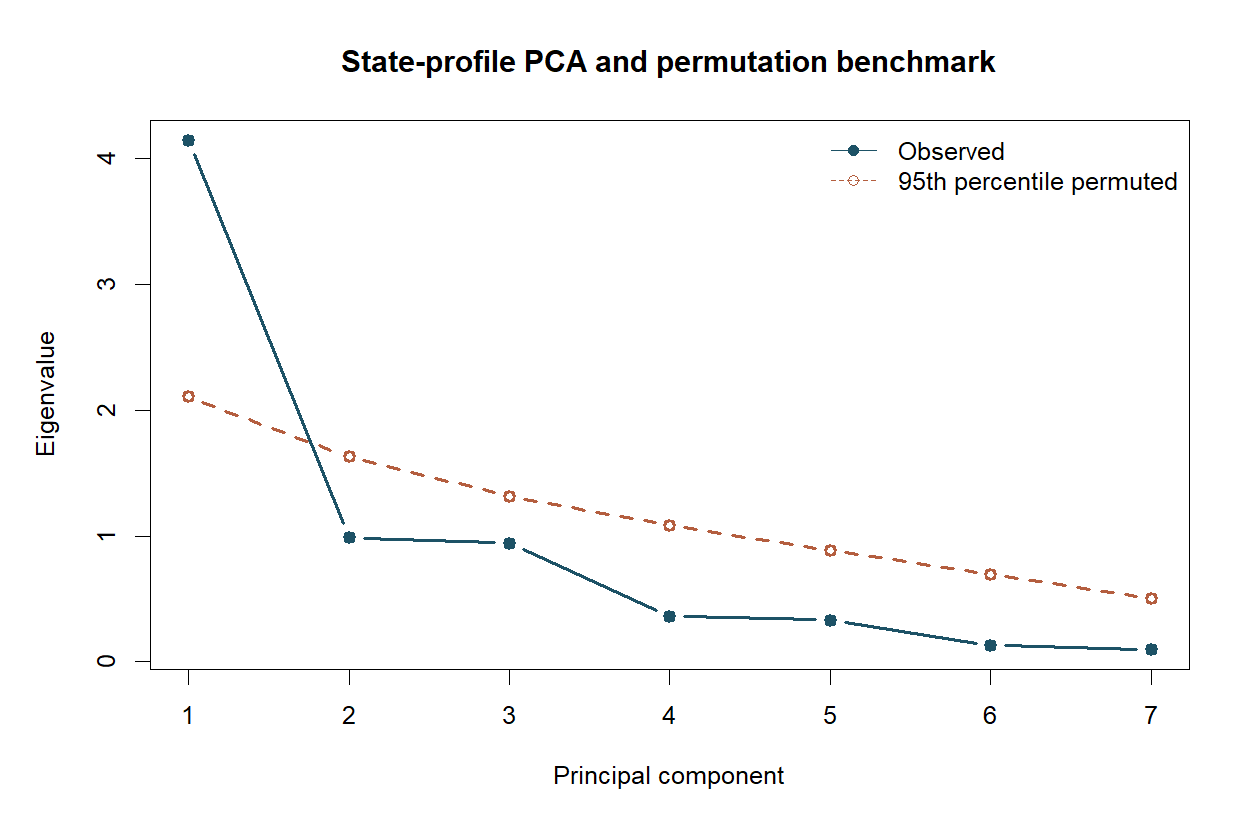
\includegraphics[width=.80\textwidth]{pca_scree_parallel.png}
\caption{Observed eigenvalues against a permutation benchmark.}
\end{figure}

\begin{figure}[H]
\centering
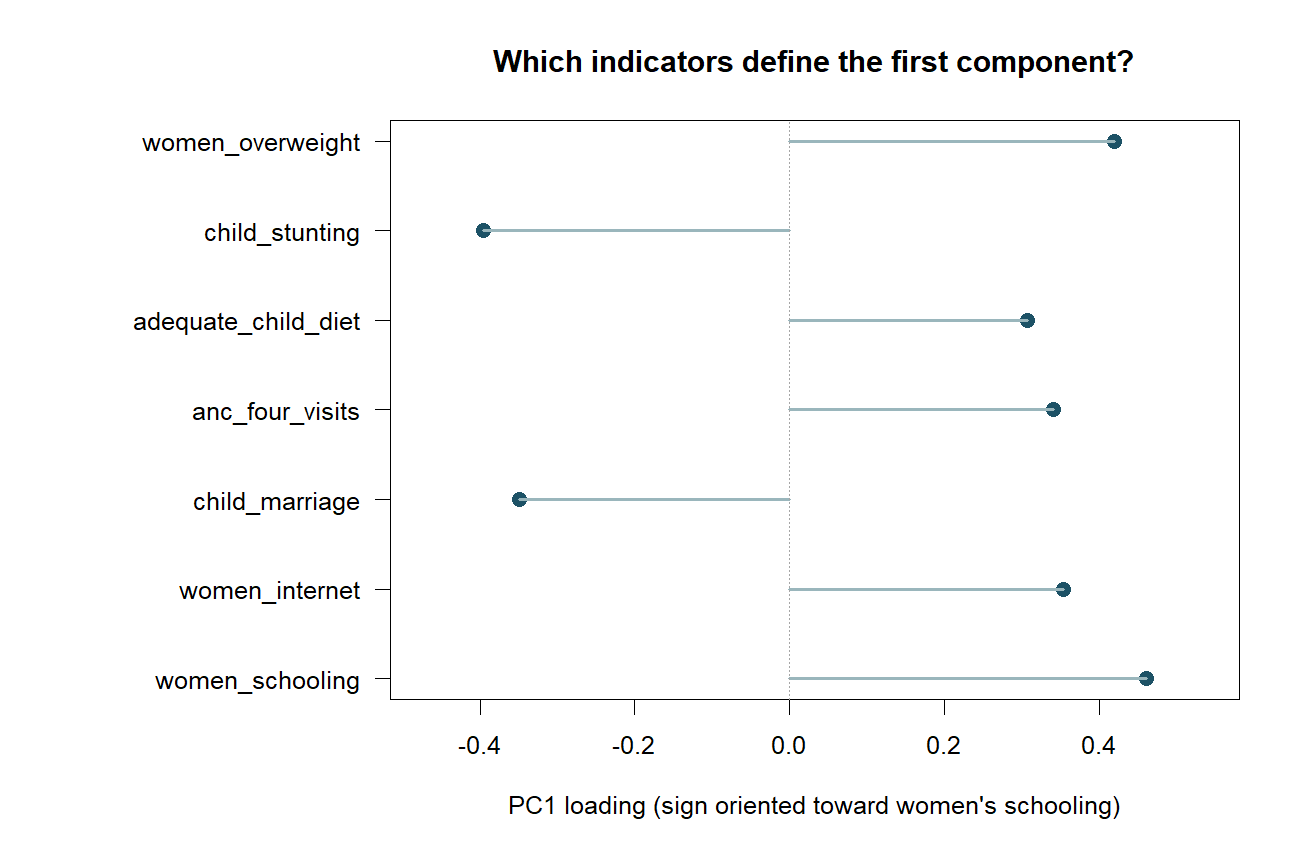
\includegraphics[width=.80\textwidth]{pca_loadings.png}
\caption{First-component loadings on standardized state indicators.}
\end{figure}

\begin{figure}[H]
\centering
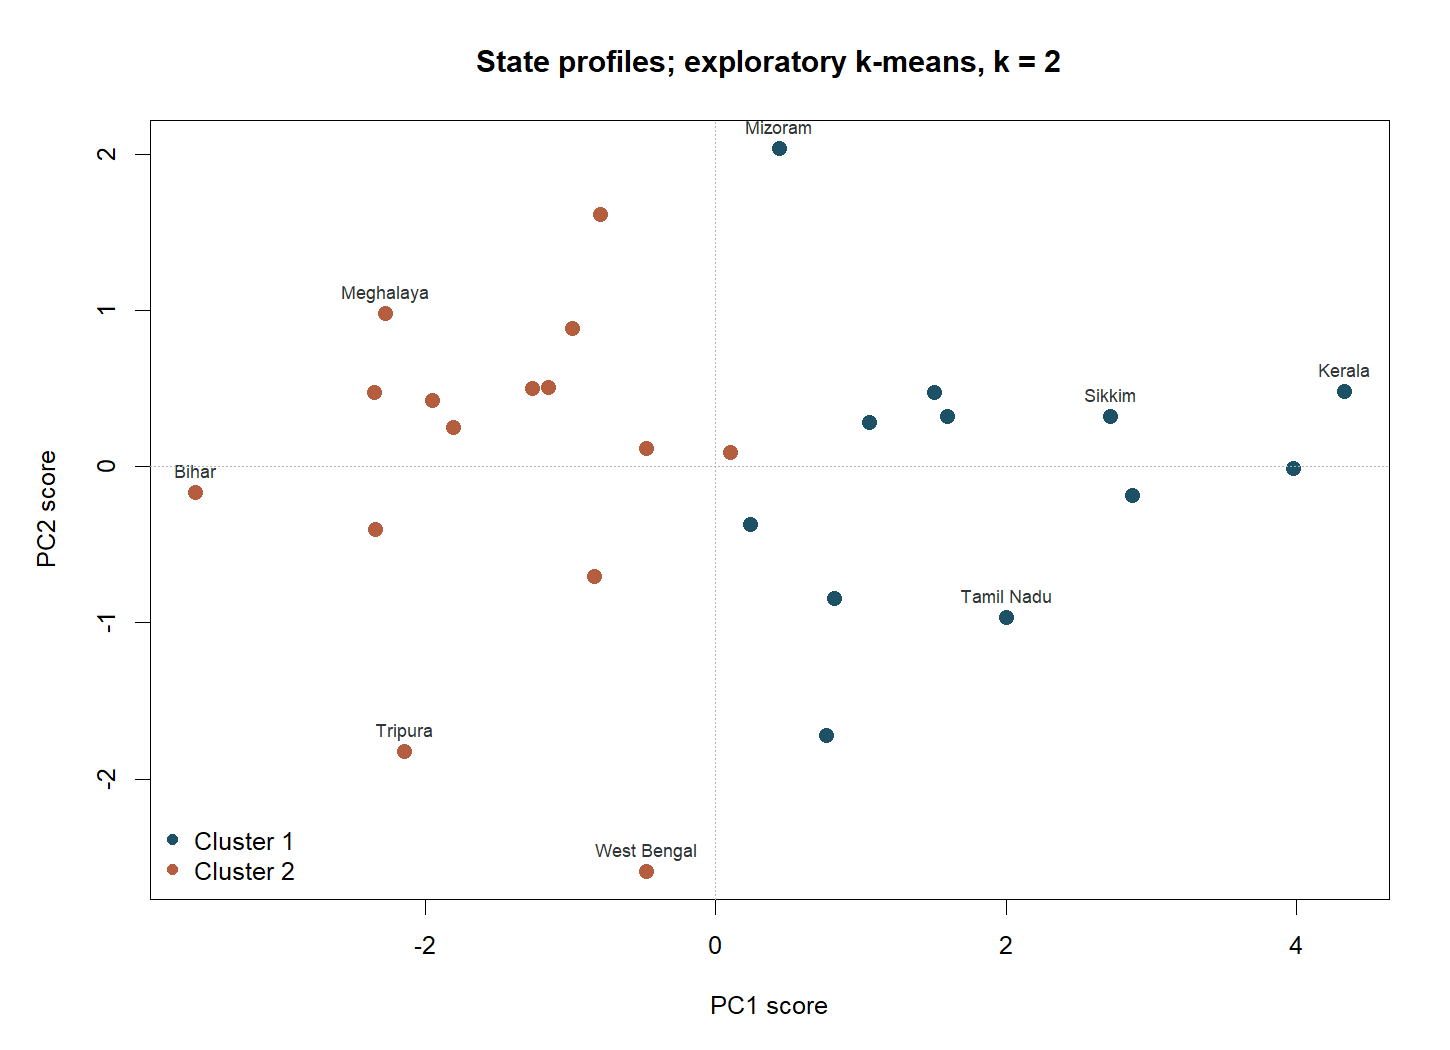
\includegraphics[width=.80\textwidth]{state_pca_clusters.png}
\caption{State scores projected on the first two components. Only selected
states are labelled for legibility; the full membership is in the CSV.}
\end{figure}

\begin{figure}[H]
\centering
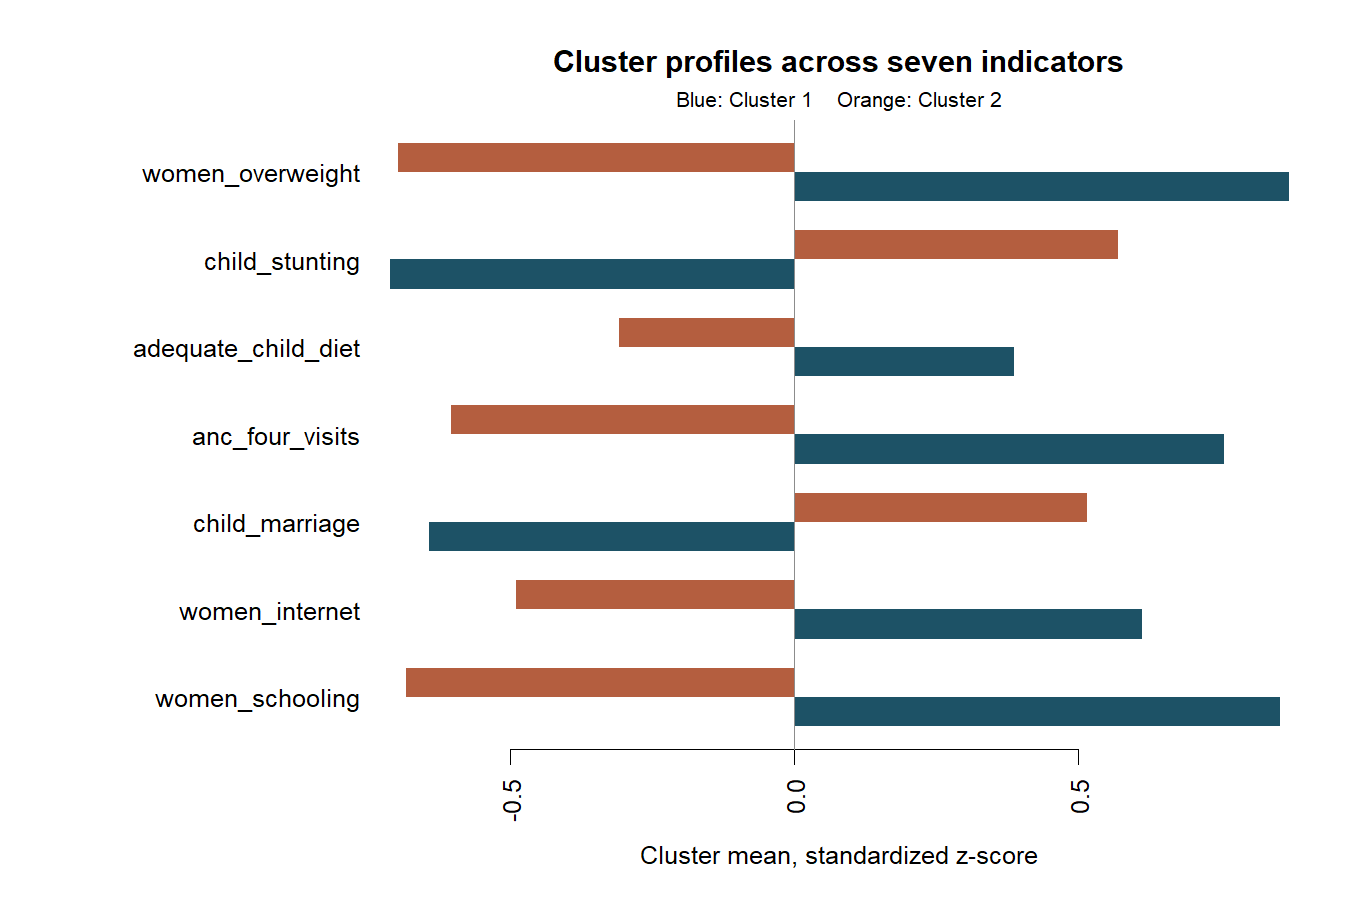
\includegraphics[width=.80\textwidth]{cluster_profiles.png}
\caption{Mean standardized indicator values by exploratory cluster.
Clustering used all seven variables.}
\end{figure}

\section{Instrumental-variable feasibility}

An IV for schooling would need relevance, independence from
unobserved determinants of stunting, and an exclusion restriction
under which it affects stunting only through schooling. The
contemporaneous NFHS area averages provide no credible externally
assigned instrument. Electricity, internet use and health insurance
can affect health or household resources directly; fieldwork phase
confounds geography with timing and possible seasonality. Schooling
would also be an implausible instrument for marriage in a teenage
pregnancy model because it may affect pregnancy through other
channels. A first-stage F statistic checks only relevance; it cannot
establish independence or exclusion. No 2SLS coefficient is reported.
The repository's IV note documents this audit and the requirements
for a future design with external policy variation.

PCA and clustering require no IV exogeneity assumption because they
estimate no treatment effect. Their quality depends instead on
indicator comparability, transparent feature choices,
standardization, missingness checks and stability. The included
code reports these checks.

\section{Limits and next steps}

All four regressions are ecological. Indicators often refer to
different people, ages or survey windows, and urban and rural
populations may differ in many unmeasured ways. HC3 does not account
for survey sampling uncertainty behind the published percentages.
The fits are exploratory after considering multiple questions and
model forms. The Q3 quadratic needs validation on new data before
being treated as a stable nonlinear relationship.

A stronger follow-up would assemble separately released NFHS-5
and NFHS-6 district fact sheets,\footnote{\url{https://www.nfhsiips.in/nfhsuser/release-details.php}}
harmonize changed district boundaries, verify matched definitions
and estimate district first differences with state effects. Even
that would be associational without a credible treatment and
comparison design. The IIPS portal stated that NFHS-6 individual
microdata were unavailable as of 30 September 2026.\footnote{\url{https://www.nfhsiips.in/nfhsuser/datarequest.php}}

From the project root, run \texttt{Rscript R/00\_run\_all.R}.
It regenerates estimates, descriptive tables, PCA and cluster
diagnostics, graphs and rendered R result images.

\end{document}
